\documentclass[9pt]{article}
\usepackage{array}
\newcolumntype{P}[1]{>{\centering\arraybackslash}p{#1}}
\usepackage{graphicx}
\usepackage{hyperref}
\usepackage{subfig}
\usepackage[parfill]{parskip}
\usepackage{float}
\usepackage[margin=1in,includefoot]{geometry}
\usepackage{fancyhdr}
\pagestyle{fancy}
\fancyfoot{}

\begin{document}

\begin{titlepage}
\begin{center}
\begin{figure}[t]
\hspace*{0.35cm}
\includegraphics[width=1.0\textwidth]{uclLogo}\\
\end{figure}
\line(1,0){300}\\
[0.25in]
\huge{\bfseries Simplicial Complex Modeling of Molecular Interactions \& Geometrical Analysis}\\
[2mm]
\line(1,0){200}\\
[1.5cm]
\textsc{\LARGE University College London}\\
\textsc{\normalsize Department of Computer Science}\\
\textsc{\normalsize COMP3096 - Research Group Project}\\
[5cm]
\end{center}

\end{titlepage}

\newpage
\section{Abstract}\label{sec:abstract}
Through comparing the representation of biological functions in the form of PPI networks and simplicial complexes, we aim to find a combination of topological factors that can predict gene description since this later affects protein functions as genes provide the instructions for protein formation. The purpose of our project extends beyond finding the correlation coefficient that best allows us to find a biological feature that can be described by a combination of topological features, and pushes us into analysing the and comparing the prediction power of both the kinds of networks explored. Understanding the role of network properties helps our chances of better understanding the biological functions of genes, and will ultimately aid in isolating causes for gene mutation and disease-causing phenotypes.

\section{Introduction}\label{sec:Introduction}
Genes are units of genetic information found in DNA, and contain instructions for building vital macro molecules known as proteins. Proteins contribute to crucial processes including transportation of molecules in cells, and catalysing metabolic reactions. The notion of protein function is very context-sensitive, but commonly described as an umbrella-term for all types of processes that a protein can be involved in, such as cellular, molecular, or physiological processes [6]. Consequently, protein function prediction explores the methods employed by bioinformatics researchers to assign such functions to poorly-studied proteins. Furthermore, these methods can provide important benefits in various ways, such as improving understanding of disease, since alterations of proteins are the cause for many diseases, and can also be used to aid rational drug design [7].
\par
Originally, many high-throughput experimental techniques, such as the yeast two-hybrid screening system (Y2H), were used to characterise protein-protein interaction networks (PPIs). [8] The experimental results from these techniques resulted in an abundance of large-scale biological networks that were stored and are still used today, on online databases such as STRING, BioGRID, and MIPS. [10] However, the speed at which new protein sequences were discovered was much faster than the speed at which experimental techniques could characterise them, due to inexpensive sequencing methods. This left a large number of proteins without functional annotations, and highlighted the need for more rapid computational prediction techniques that could complement and guide experimental research. [14]
\par
The first techniques for protein function prediction included homology-based methods, which describes the process of predicting a protein’s function based on similarities in amino acid sequences.[11,12] It was a technique regularly used because strong similarities usually inferred that two proteins were related by a divergent evolution of a common ancestral gene, and thus would be similar, if not identical, in function. [13] Additionally, many older studies also began exploring the use of topological analyses of PPIs to predict protein function, such as direct annotation schemes, which infer a protein’s functions based on its connections within the network [21]. The simplest example for this category of techniques is known as neighbourhood-counting, and this predicts that proteins that are topologically close in a network will likely have similar functions. [17,19,20] Furthermore, another successfully exploited premise describes that proteins in a network that have topologically-similar neighbourhoods, often share similar functions [16,18]. 
\par
Nevertheless, the most common representation of the PPIs in these approaches use traditional graph-theory. This is partly due to the inherent simplicity for graphs in representing proteins as nodes, and interactions between proteins as edges. However, simply binary models such as graphs are not be able to fully express the higher order organizations of interactions found in protein complexes or biological pathways [1]. As a result, the intent of this study is to explore another form of data representation, simplicial complexes [30], a generalised network structure capable of modelling interactions between groups of nodes [1,22]. 
\par
Furthermore, another concept we utilise in conjunction with simplicial complexes involves applying the concept of node centrality. Centrality indices have been successfully exploited in many studies for identifying the importance of a protein with respect to its position in the PPI [1,2,3,4]. We look to see if extending these measures to simplicial complexes, will help in predicting protein function.
\par
Therefore, the purpose of our study is to investigate a fairly new way to model multi-scale protein organisation, by using simplicial complexes with a set of centrality measures, and observe if geometric descriptors of proteins in Saccharomyces cerevisiae (baker’s yeast) relate to their biological function. For comparing results, we will use the same yeast PPI, but modelled by a simple graph and analogous centrality measures.
\par
To obtain our dataset, we download the latest protein interaction data for yeast from BioGRID [23], a public database that archives protein interaction data. Furthermore, we obtain a set of yeast protein complexes catalogued in the MIPS database, known as CYC2008 [25]. We then modelled the yeast PPI by using simple graphs and simplicial complexes. In both these models, we identified and calculated three centrality measures known as degree distribution, betweenness and closeness centralities. 
\par
After doing so, we collected the biological annotations of each protein from Gene Ontology (GO) [24], a framework that describes gene functions and the relationships between them. The initiative provides an ontology of GO terms, which represent gene product properties. As a result, we mapped the genes to their corresponding vector of GO:ID, a unique identifier for each GO term, and made use of this mapping to create a 2D matrix of GO:ID and gene. Using binary notation, we then indicated whether each GO:ID is present in the annotation vector of a particular gene.
\par
Lastly, to build our models, we used Scikit-learn [29], a machine learning python library that offers a wide range of regression, clustering and classification algorithms. However, before creating the models, we decide on a cross-validation method to assess the predictive performance of the models and observe their effectiveness on independent data sets. To do this, we perform a random split of the data in an 8:2 ratio. The former of the split data is used to train the model and the latter is used for validation of the model. We then trained our models with linear regression, logistic regression, random forest classifier, and random forest regressor algorithms. 
\par
Our initial results showed that the machine learning models did not provide any statistically significant results. The results indicated that the yeast network, modelled by using a simplicial complex, was not more accurate at predicting protein function compared to a graph-based PPI in most cases. For more detailed analysis of our results, see the Results section.
\par
Therefore, we adapted our methodology to work with hierarchical agglomerative clustering (HAC) for enrichment analysis instead. HAC is a type of bottom-up hierarchical clustering technique where each gene would start as its own cluster and pairs of clusters would be merged, dependent on a similarity measure, up the hierarchy. The resulting clusters of genes would then be subject to enrichment analysis where each gene set is compared to GO terms, and a statistical test would calculate for each GO term whether it is enriched for the input genes. This analysis would then allow finding groups of genes that are over-represented in a cluster, and potentially use this knowledge to predict functions of the remaining genes in that cluster.
\par
Our final results found that the clustering, based on all three centralities in simplicial complexes, did not result in more enriched GO terms than the graph-based PPI. However, results still showed that increasing the number of clusters correlated with an increase in the number of enriched GO terms in both the graph-based PPI and simplicial complex representations.


\section{Related Work}
For studies on protein function prediction, we discovered no relatable methodologies that incorporate simplicial complexes. However, a big inspiration for our investigation can be found in a study published in the Journal of Theoretical Biology by Estrada \& Ross (2018) [1]. In this study, Estrada \& Ross extend the concept of node centrality from simple graphs to simplicial complexes. They calculate three main centrality measures (degree distribution, subgraph, and closeness) for node, edge and triangle simplices in a yeast network. One of the outcomes when they studied the correlations between centrality measures was that the centralities at different simplicial levels had a lot of variation and did not necessarily agree with each other. This knowledge is useful for future studies, like ours, since we happen to use two of the three same centrality measures, being degree distribution and closeness, on a yeast PPI too. However, the main difference between our methodologies is that we hope to extend centralities to simplicial complexes to aid protein function prediction, as opposed to identifying essential proteins.
\par
Additionally, there have been previous studies that similarly implemented clustering-based algorithms for enrichment analyses of PPIs. Tedder et al (2010) [32] create a program, PAGODA (Protein Assignment by Gene Ontology Data Associations), which uses semantic similarity clustering and enrichment analysis algorithms to predict gene functions in malaria parasite Plasmodium falciparum. However, a big decision in using clustering-based methods is the choice of similarity measure between pairs of proteins, since this ultimately decides the types of clusters that are formed, and thus used in enrichment analysis

\section{Research Hypothesis}
Our research hypothesis is that “The accuracy of protein function prediction is higher using the correlations provided by the combination of both PPI graph and simplicial complex data representations rather than PPI graphs alone”. 

\section{Dataset Description/Data Collection}
In this section we will be defining the origin of our data sets as well as tools used for conversions of such data within our data cleaning process. As stated previously our focus has been in collecting data from saccharomyces cerevisiae as they are the most complete dataset.

\subsection{BioGRID \& CYC2008}
Biological General Repository for Interaction Datasets (BioGRID)[23] is an online repository for protein and genetic interactions. Its aim is to provide a comprehensive curated resource for all major species, such as homo sapiens and saccharomyces cerevisiae. Additionally, CYC2008 [25] provides an up-to-date reference set of yeast protein complexes which we have used in our experiments. 

\section{Methodology}
\subsection{Data Cleaning}
Data cleaning was the first methodology we tackled to correct inaccurate records to increase the accuracy of our data as much as possible. We faced many issues regarding data uniformity, data duplication, data conversion and inaccurate or irrelevant fields within the data sets. 
\par
To minimise the effect of such problems, we used the most standardised databases for interaction datasets including: BioGRID (PPI networks), CYC2008 \& CORUM (Complexes networks), Gene Ontology (Biological annotations), as well as tools such bioDBnet for Gene ID conversion. More specifically, we have cleaned the data by only considering the experimental derived PPI’s to be only “Physical”. However, it important to note that even after cleaning the data we only have access to high throughput physical interactions, which are still very noisy due to biotechnological limitations and human bias

\subsection{Protein-Protein Interaction Networks and Simplicial Complexes}
After data cleaning, we proceeded in exploring different methodologies for the creation of PPI and Simplicial Complexes networks. We decided to use well established Python packages for PPI networks, as well as custom made packages specifically for simplicial complexes.
\par
For the making of the PPI networks we used NetworkX [31]., which is a Python package “for the creation, manipulation, and study of the structure, dynamics and functions of complex networks”. Some of the key features of this package were: Data structures for graphs, digraphs and multigraphs, many standard graph algorithms and network structure and analysis measure, which will be explored in the next section.However, for the creation of simplicial complexes networks we implemented our own networks since no such libraries exist. 

\subsection{Centrality Measures}
Within network analysis and graph theory, centrality measures identify the most valuable nodes within a graph [37]. Centrality measures ultimately tries to answer the question of  “what characterises an important node?”. From this measurement of centrality we can get an idea of the importance of a node within a given network, therefore we decided to both use libraries available to calculate the centrality measurements as well as implementing them from scratch. A complexity analysis of centrality measures will be discussed later in this report. Some of the key centralities explored are explained below

\subsubsection{Degree Centrality}
A simple measure that counts how many neighbours a node has. The degree centrality of a node of a node \(n\), for a given graph \(G:=(N,E)\) with \(|N|\) nodes and \(|E|\) edge is defined as \(C_D(V) = deg(v)\) [ref]. 

\subsubsection{Closeness Centrality}
A measure of the degree to which a node is near all other nodes in a network. It is calculated as the sum of the length of the shortest paths between the node and all other nodes in the graph. Therefore, if a node is more central, this means that it is closer to all the other nodes. More concretely closeness centrality is defined as the reciprocal of the sum of the shortest path distances from \(u\) to all \(n-1\) other nodes. “As the sum of distances is dependent on the number of nodes in the graph, closeness is normalised by the sum of minimum possible distances \(n-1\),  where \(d(u, v)\) is the shortest-path distance between \(u\) and \(v\), and \(n\) is the number of nodes in the graph” [38]. 
\begin{equation}
C(u)=\frac{n-1}{\sum_{v=1}^{n-1} d(v,u)}
\end{equation}

\subsubsection{Betweenness Centrality}
Betweenness centrality of a node \(v\) is the sum of the fraction of all-pairs shortest paths that pass through \(v\) [39]:
\begin{equation}
C_B(v)=\sum_{s,t\in{V}}\frac{\sigma(s, t|v)}{\sigma(s, t)}
\end{equation}
“Where \(V\) is the set of nodes, \(\sigma(s, t)\) is the number of shortest \((s, t)\) paths, and \(\sigma(s, t|v)\) is the number of those paths passing through some node \(v\) other than \(s\), \(t\). If \(s = t\), \(\sigma(s, t) = 1\), and if \(v \in (s, t), \sigma(s, t|v) = 0\)”.

\subsection{Annotation Vectors}
We used data collected from Gene Ontology to map the relevant genes to their GO annotation, which described the function of the gene [24].
In order to discard information that weren’t from experimentally valid sources, we traverse the column of genes, we also check its corresponding column vector and ensure that the Evidence ID belongs to list of ID’s from under ‘Experimental Evidence codes’ which shows that the GO term has been supported by physical characterization of the gene or gene product [24] as we cannot work with predicted data.Therefore it has to be one of the following: Inferred from Experiment (EXP), Inferred from Direct Assay (IDA), Inferred from Physical Interaction (IPI), Inferred from Mutant Phenotype (IMP), Inferred from Genetic Interaction (IGI) and Inferred from Expression Pattern (IEP) [24]. Using the mapping between genes and its corresponding GO:ID vectors, we constructed a matrix with binary values to indicate whether the selected GO:IDs were present in the gene’s vector or not.

\subsection{Machine Learning Models}
We decided to explore a variety of machine learning models, starting from the simplest and experimenting with more complex algorithms as we progressed In order to build our models, we used scikit-learn which is a free machine learning python library which offers a wide range of regression, clustering and classification algorithms [29]. The core algorithms in this library are written in Cython to achieve performance. The machine models used are explained in more detail below. 

\subsubsection{Linear Regression}
For our first experiment, we decided to train a model with linear regression. We simply wanted to test and explore this methodology for the unlikelihood of obtaining meaningful results even though linear regression is not suitable for our purpose. Linear regression is a linear approach to model the relationship between a scalar output variable \(y\) and one or more explanatory input variables \(x\). The linear equation, assigns a certain coefficient to each input variable. For example, a single input variable linear regression equation would look like $y = B_0 + B_1\times{x}$, where \(B_1\) is the coefficient for input \(x\) and \(B_0\) is the bias coefficient giving the line the freedom to move up and down: 

In our experiment, since we wanted to model the data with not only each centrality, but also all the combinations of centralities, we used multivariable linear regression, which the form of the model would be a plane or a hyper-plane:
\begin{equation}
y=B_0 + B_1\times{x} + B_2\times{y} + B_3\times{z}  
\end{equation}
(\(x\) = degree distribution, \(y\) = closeness centrality, \(z\) = betweenness centrality)

Learning the model using linear regression means estimating the coefficient using the data we have available for training. There are different techniques for learning the linear regression model. The most commonly used one is Ordinary Least Square, which scikit-learn linear regression uses

\subsubsection{Logistic Regression}
We also used Logistic Regression as part of one of our experiments to train another model. The idea behind logistic regression is same as linear regression, except that the outcome is binary. This means that the only two possible outcomes can be 0 (FALSE) or 1 (TRUE) and the outcome is based on the probability of the presence of the characteristic of interest. This method seemed to be well suited for our dataset and what we wanted to predict, since a gene is either annotated with a GO id or not. 

\subsubsection{Random Forest}
Additionally, we used random forest, which is a type of ensemble modelling. Ensemble modelling is a divide and conquer approach to improve performance. The idea behind ensemble modelling is that there are some weak learners and one strong learner. The result from the weak learners will be used to train the strong learner. The Random Forest algorithm starts off by a decision tree which is a weak learner, the algorithm then builds the strong learner that is the random forest by combining the trees (weak learners).

\subsubsection{Hierarchical Agglomerative Clustering}
Lastly, we attempted hierarchical agglomerative clustering which is a bottom up approach where each observation start within their own clusters and pairs of clusters are merged into new clusters as one moves up the hierarchy. To be able to correctly decide which clusters are combined with each other a measure between the sets are required. 

This is achieved by choosing a suitable metric such as a measure of distance between the pairs, in our case the Euclidean distance. A appropriate metric will impact the shape of the clusters, since some elements may be close to each other to one distance but farther away from another. Additionally, a linkage basis is required, a linkage “specifies the dissimilarity of sets as a function of the pairwise distances of observations in the sets”, in our case it is the Ward’s method.  Using clustering we performed an enrichment analysis, which is a method to identify classes of proteins that are over represented or underrepresented using annotations for that gene set. 

\subsection{Benchmarks}
No reasonable benchmarks except possibly comparing spearman’s rank correlation coefficients with Estrada paper. Even still they use an entirely different dataset as well as a slightly different methodology. It is important to note that the purpose of this paper is to experiment on soley new ideas and methodologies that have not been done in the past, thus finding out new results.  

[Needs to be re-written nicely]
For building proteins as simplicial complexes, no reasonable benchmarks exist. The only existing method(s) that bears resemblance are the other HAC or even other forms of clustering methods, for gene enrichment analysis. 
For PPI, *look through the papers and see if any of them have a different score to us?*

\newpage
\section{Analysis of Results}
\subsection{Linear Regression}
{
\begin{center}
\begin{tabular}{ |P{5cm}||P{5cm}|}
 \hline
 \multicolumn{2}{|c|}{Linear Regression} \\
 \hline
Combination of Centralities &Average mean squared error across all Go-ids\\
 \hline
(0, 1) PPI   &0.001211887408350228\\
(0, 1) SIMP & 0.0012126315661762492\\
(2,) PPI &0.0012127442848385173\\
(2,) SIMP &0.0012112071926545654\\
(0, 2) PPI &0.0012127048064502438\\
(0, 2) SIMP &0.001210476789533034\\
(0, 1, 2) PPI  &0.0012118307398820312\\
(0, 1, 2) SIMP &0.0012110116447171836\\
(1, 2) PPI &0.0012132378607974665\\
(1, 2) SIMP &0.0012115913303623323\\
(0,) PPI &0.0012129864311300038\\
(0,) SIMP &0.0012120214216284723\\
(1,) PPI &0.0012137853300388825\\
(1,) SIMP &0.0012131195409431218\\
 \hline
\end{tabular}
\end{center}
As we can see, Regression is not ideal for this problem. All the models we generated using regression have a really low prediction capacity and really high error rate. Since the problem we are dealing with is a classification problem, regression models are expected to perform poorly. To train our model, we have taken all the combinations of centralities. In the above table, the tuples show what combinations we have used with \(0\) being betweenness centrality, \(1\) being closeness centrality and \(2\) being degree distribution. 

\subsection{Logistic Regression}
\begin{figure}[!htb]
\minipage{0.32\textwidth}
  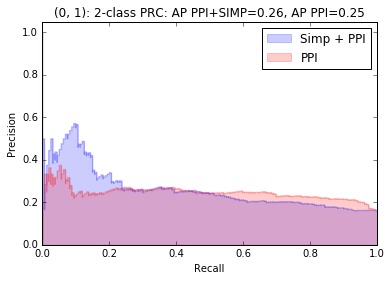
\includegraphics[width=\linewidth]{logisticRegressionGraphs/logr1.png}
\endminipage\hfill
\minipage{0.32\textwidth}
  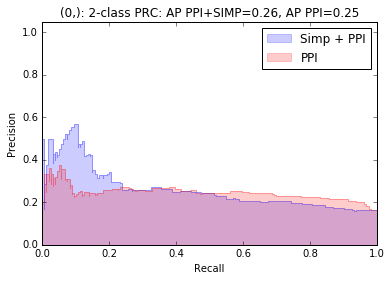
\includegraphics[width=\linewidth]{logisticRegressionGraphs/logr3.png}
\endminipage\hfill
\minipage{0.32\textwidth}%
  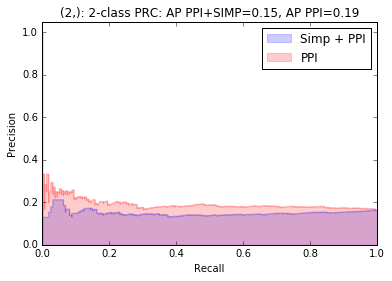
\includegraphics[width=\linewidth]{logisticRegressionGraphs/logr6.png}
\endminipage
\end{figure}
What above figures show, is the difference Precision and Recall curves for different combination of input and how the resulted logistic regression model performed in both ppi and simplicial complexes network. As we can notice, our maximum average precision over all the combination of input is 25\% in simplicial complexes and 22\% in PPI networks. Something else we can observe is that our precision drops really suddenly once we increase the recall. Which means, only very few instances are right if we want to be precise. Precision drops to a constant value and stays around it as the recall increases. It is clear that prediction capacity of this model is quite bad. Some combinations seems to perform better under simplicial complexes and some combinations performs worse.

\newpage
\begin{figure}[!htb]
\minipage{0.32\textwidth}
  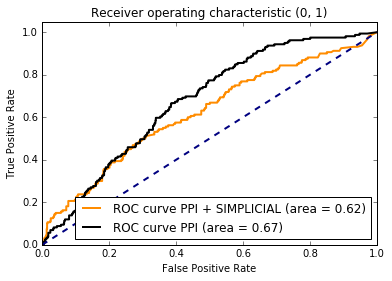
\includegraphics[width=\linewidth]{logisticRegressionGraphs/logr1S.png}
\endminipage\hfill
\minipage{0.32\textwidth}
  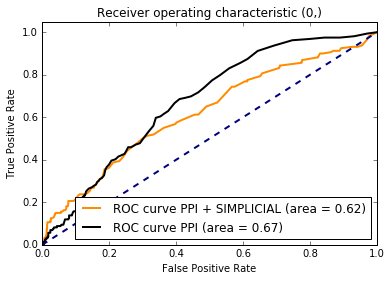
\includegraphics[width=\linewidth]{logisticRegressionGraphs/logr2S.png}
\endminipage\hfill
\minipage{0.32\textwidth}%
  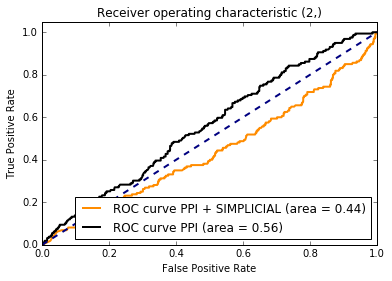
\includegraphics[width=\linewidth]{logisticRegressionGraphs/logr3S.png}
\endminipage
\end{figure}
Above shown Receiver Operating Characteristic (ROC) are plotted based on the combination of models we generated from different combinations of input. The dotted line represents the True and False positive output we get from a random classifier when we move the threshold of the prediction from high to low. The Orange curve, ROC curve, represents the True and False positive rate we would get from the models as we move our threshold. Even though three out of 7 models perform bit better than a random classifier, these model’s prediction power is quite low and have a high False positive rate. As we can see, some of the combinations have better True and False positive rate considering the area under the curve which shows how good a model performs. (First and third models have the area value of 0.66 which is more than the other combinations)

\subsection{Random Forest Classification}
\begin{figure}[!htb]
\minipage{0.32\textwidth}
  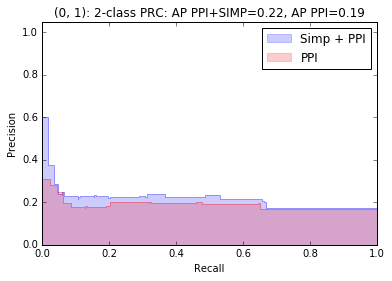
\includegraphics[width=\linewidth]{logisticRegressionGraphs/for1.png}
\endminipage\hfill
\minipage{0.32\textwidth}
  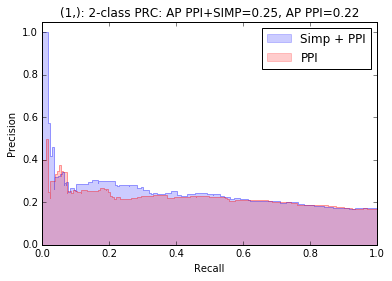
\includegraphics[width=\linewidth]{logisticRegressionGraphs/for2.png}
\endminipage\hfill
\minipage{0.32\textwidth}%
  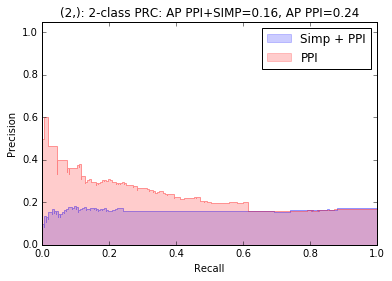
\includegraphics[width=\linewidth]{logisticRegressionGraphs/for3.png}
\endminipage
\end{figure}

Above figures depict different Precision and Recall curves for different combination of centrality inputs and how Random Forest Classification model performed in both ppi and simplicial complexes networks. According to the figures, maximum average precision over all the combinations of centralities as inputs is less than 20\% in ppi networks and simplicial complexes around 20\%. Also it is important to note that, some models seems to have a slower drop in precision in both Simplicial Complexes and PPI networks. We can see that simplicial complex models only perform better under certain combination of topological measures but the maximum average precision suggest that this enhancement in performance is not significant. For all the models, the precision barely increases as the recall increases and it’s almost constant after a certain recall in PPI networks.

\newpage
\begin{figure}[!htb]
\minipage{0.32\textwidth}
  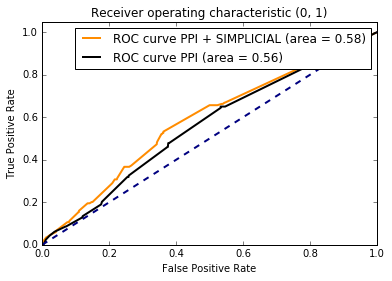
\includegraphics[width=\linewidth]{logisticRegressionGraphs/forS1.png}
\endminipage\hfill
\minipage{0.32\textwidth}
  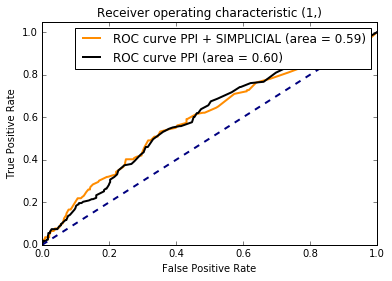
\includegraphics[width=\linewidth]{logisticRegressionGraphs/forS2.png}
\endminipage\hfill
\minipage{0.32\textwidth}%
  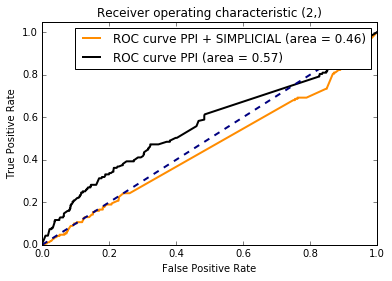
\includegraphics[width=\linewidth]{logisticRegressionGraphs/forS3.png}
\endminipage
\end{figure}
ROC curves for Random Forest Classification shows the similar performance, if not worse compared to the one we got for Logistic regression. On average, random forest classification gives us worse performance and worse average area under the curve. Also we can note that simplicial complexes do not perform better in some combinations of inputs as measures.

\subsection{Agglomerative Clustering}
\begin{figure}[!htb]
  \centering
  \minipage{0.7\textwidth}%
  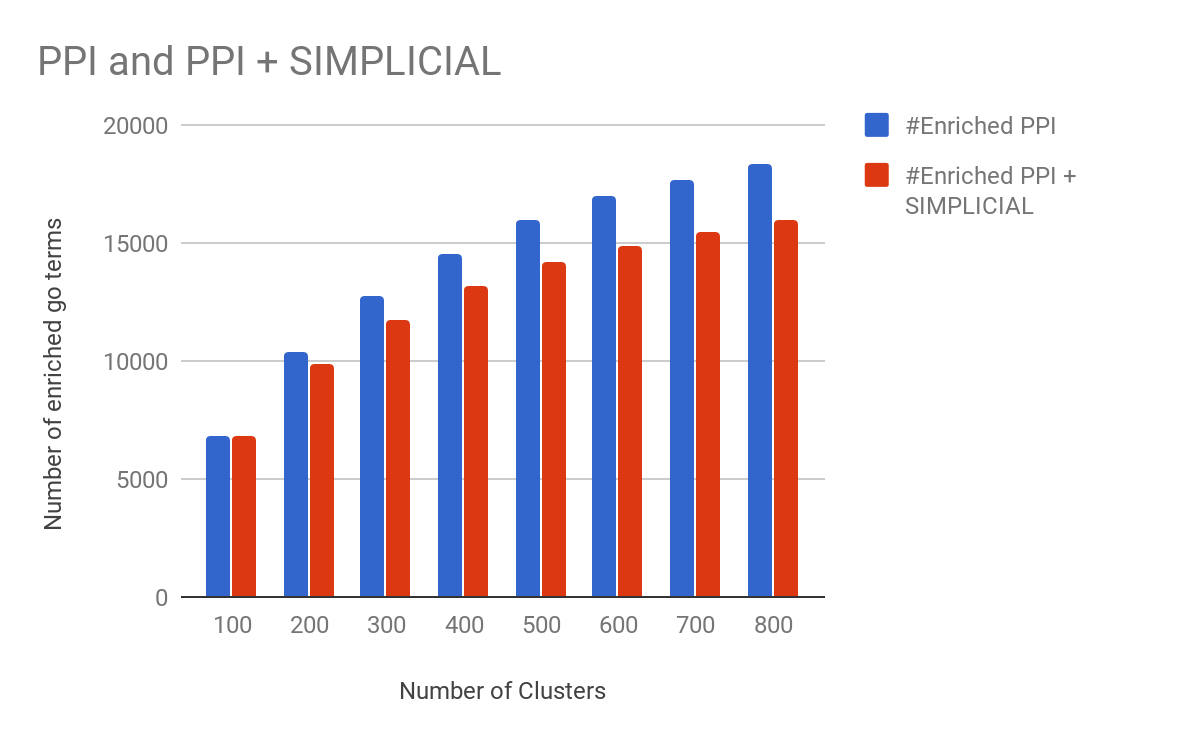
\includegraphics[width=\linewidth]{logisticRegressionGraphs/cluster.png}
\endminipage
\end{figure}
We applied agglomerative clustering on the genes centrality data that we have collected on both ppi and simplicial complexes. We analysed each cluster to see if any of the GO terms are enriched in them. We calculated the p value for each GO term in each cluster for both ppi and simplicial complexes.\url{(https://www.nature.com/articles/srep35098\#supplementary-information)} We repeated the experiment by changing the number of clusters from 100 - 800 incrementing by 100 every time. The above figure depicts the number of clusters we have in the experiment and the number of enriched GO terms in that experiment. As we can see clustering based on all three centralities (betweenness, closeness and degree distribution) in simplicial complexes, did not give us more enriched GO terms. The figure also shows that as we increase the number of clusters, the number of enriched GO terms increases in both PPI and simplicial complexes. For future, this clustering may be used for predicting GO terms in the clusters. Also we can use combinations of centralities for our clustering model in future to see if we get better enrichments in both simplicial complexes and ppi networks. 

\section{Discussion \& Limitations} 
After putting the complexes network on top of PPI network, in order to build the simplicial complex, we had around 65,000 - 75,000 triangles (nodes) in the network. For us to compute closeness centrality and betweenness centrality, we needed to calculate the shortest paths between each pair of triangles. As Floyd Warshall’s shortest path algorithm is $O(N^3)$, and the number of edges in the simplicial complexes is well over 150 million, it is computationally exhaustive to calculate. A naive implementation could take easily 11 days for betweenness centrality to complete. Also as all the algorithms we implemented were in python, which is a higher level language with a lot more abstractions, it is in fact much slower than other lower level languages.

To address this issue, instead of using our own implementation of centralities and shortest path algorithms for simplicial complexes, we used NetworkX library. In order for us to use this library, we had to model our triangular network as a binary network, which means that each triangle in the network would be considered a node and the edge list would be built accordingly. This made the calculation significantly faster because of the optimisation already applied in NetworkX implementations being done in C and C++.

Additionally, another limitation arose as we had no access to any powerful computer clusters therefore, we were unable to continuously run our experiments as they became extremely time consuming to process. However, as well as having access to power clusters, since this project is very heavy data driven, parallelisation can be an effective methodology to speed up the computations required.   

\section{Conclusion and Future Work}
Our experiments and follow up analysis show that simplicial complexes can have a effect 
on predictiveness power of the models we generate by adding a layer on simplicial complex on top of PPI comparing to just bare PPI network. 

Main limitations of this experiment was the sheer amount of data to filter through and multiple layer of filtering actually limited us in the possible varieties of machine learning models we could have used. Since we are using python, the computation time has increased at least 5x. We could reduce this by implementing time computation sensitive parts in faster low level languages such as C/C++ or Java. To give a perspective on the time and space constraints in order to calculate the metrics we used in this experiment, for a simplicial complex, there are ~200 million edge between nodes, where each nodes are a n sided polygon. Our experiment is based on 3 sided polygons, triangles, which resulted in having around 154,000,000 edges between the nodes. As we go higher in the dimensions, the number of edges would increase exponentially making it computations infeasible to approach. So we limited ourselves in calculating only up to triangles in a simplicial complex. 

Filtering of data through multiple processes have actually thrown lots of data away. After initial processing and calculation of metrics, we find the intersection of all the genes that are annotated with the genes whose metrics we have in order to build models, so this reduces the possible data points we have significantly. Hence not being able to use certain methodologies such as Neural network to make predictions.

Future work on this can begin by implementing higher dimensions of simplicial complexes. This would give us more metrics and can be used in combinations to find a model that would have higher prediction capacity. 



\newpage
\begin{thebibliography}{8}
\bibitem{latexcompanion} 
Estrada, E. and Ross, G. (2018)
Centralities in simplicial complexes. Applications to protein interaction networks. Journal of Theoretical Biology, 438, pp.46-60

\bibitem{latexcompanion} 
Hahn, M. and Kern, A. (2004)
Comparative Genomics of Centrality and Essentiality in Three Eukaryotic Protein Interaction Networks. Molecular Biology and Evolution, 22(4), pp.803-806.

\bibitem{latexcompanion}
del Rio, G., Koschützki, D. and Coello, G. (2009). 
How to identify essential genes from molecular networks?. BMC Systems Biology, 3(1), p.102.

\bibitem{latexcompanion}
Chapter 4 of “Analysis of Biological Networks,“ edited by Bjorn J. Junker and Falk Schreiber, John Wiley \& Sons, 2008 

\bibitem{latexcompanion}
Wrzeszczynski, K., Ofran, Y., Rost, B., Nair, R. and Liu, J. (2003). Automatic prediction of protein function. Cellular and Molecular Life Sciences (CMLS), 60(12), pp.2637-2650.
 
\bibitem{techPapers} 
Cs.umn.edu. (2018). Browse Technical Reports, Computer Science \& Engineering. [online] Available at: \url{https://www.cs.umn.edu/research/technical_reports/view/06-028l} 

\bibitem{techWebsite}
Semanticscholar.org. (2018). A (not so) Quick Introduction to Protein Function Prediction - Semantic Scholar. [online] Available at: \url{https://www.semanticscholar.org/paper/A-(not-so)-Quick-Introduction-to-Protein-Function-Radivojac/d678f9a5e6e430b165b6a98f5fac2cfe66c3dc7c}

\bibitem{techwebsite}
Young, K. (2018). Yeast Two-hybrid: So Many Interactions, (in) So Little Time….
\url{https://academic.oup.com/biolreprod/article/58/2/302/2761050}

\bibitem{latexcompanion}
Gligorijević, V., Barot, M. and Bonneau, R. (2017). deepNF: Deep network fusion for protein function prediction. biorxiv preprint doi:10.1101/223339

\bibitem{latexcompanion}
Yu, D., Kim, M., Xiao, G. and Hwang, T. (2013). Review of Biological Network Data and Its Applications. Genomics \& Informatics, 11(4), p.200.

\bibitem{latexcompanion}
Andrade, M., Casari, G., de Daruvar, A., Sander, C., Schneider, R., Tamames, J., Valencia, A. and Ouzounis, C. (1997). Sequence analysis of the Methanococcus jannaschii genome and the prediction of protein function. Bioinformatics, 13(4), pp.481-483

\bibitem{latexcompanion}
Reeck, G. R.; de Haen, C.; Teller, D. C.; Doolittle, R. F.; Fitch, W. M.; Dickerson, R. E.; et al. (1987). ""Homology" in proteins and nucleic acids: a terminology muddle and a way out of it". Nature. 50 (5): 667.

\bibitem{latexcompanion}
EMBL-EBI Train online. (2018). Protein Classification. [online] Available at: \url{https://www.ebi.ac.uk/training/online/course/introduction-protein-classification-ebi/protein-classification}.

\bibitem{latexcompanion}
Zhao, H. (2018). Protein function prediction by integrating sequence, structure and binding affinity information. [online] Scholarworks.iupui.edu. Available at: \url{https://scholarworks.iupui.edu/handle/1805/3913}

\bibitem{latexcompanion}
Davis, D., Yaveroğlu, Ö., Malod-Dognin, N., Stojmirovic, A. and Pržulj, N. (2015). Topology-function conservation in protein–protein interaction networks. Bioinformatics, 31(10), pp.1632-1639.

\bibitem{latexcompanion}
Milenković T. Pržulj N. (2008) Uncovering biological network function via graphlet degree signatures. Cancer Inform. ,2008, 257–273.

\bibitem{latexcompanion}
Schwikowski, B., Uetz, P. and Fields, S. (2000). A network of protein–protein interactions in yeast. Nature Biotechnology, 18(12), pp.1257-1261.

\bibitem{latexcompanion}
Przulj N, Wigle DA, Jurisica I (2004) Functional topology in a network of protein interactions. Bioinformatics 20: 340–348

\bibitem{latexcompanion}
Chua, H., Sung, W. and Wong, L. (2006). Exploiting indirect neighbours and topological weight to predict protein function from protein-protein interactions. Bioinformatics, 22(13), pp.1623-1630.

\bibitem{latexcompanion}
Hishigaki, H., Nakai, K., Ono, T., Tanigami, A. and Takagi, T. (2001). Assessment of prediction accuracy of protein function from protein-protein interaction data. Yeast, 18(6), pp.523-531.

\bibitem{latexcompanion}
Sharan, R., Ulitsky, I. and Shamir, R. (2007). Network-based prediction of protein function. Molecular Systems Biology, 3.

\bibitem{latexcompanion}
Courtney, O. T., \& Bianconi, G. (2016). Generalized network structures: The configuration model and the canonical ensemble of simplicial complexes. Physical Review E, 93(6), 062311. 

\bibitem{latexcompanion}
Lab, M. (2018). BioGRID | Database of Protein, Chemical, and Genetic Interactions. [online] Thebiogrid.org. Available at: \url{https://thebiogrid.org/}

\bibitem{latexcompanion}
Gene Ontology Consortium (2018). The Gene Ontology (GO) database and informatics resource.

\bibitem{latexcompanion}
Wodaklab.org. (2018). About - CYC2008 - Wodak Lab. [online] Available at: \url{http://wodaklab.org/cyc2008/}

\bibitem{latexcompanion}
P. Tedder, J. Bradford, C. Needham, G. McConkey, A. Bulpitt and D. Westhead, "Gene function prediction using semantic similarity clustering and enrichment analysis in the malaria parasite Plasmodium falciparum", Bioinformatics, vol. 26, no. 19, pp. 2431-2437, 2010.

\bibitem{latexcompanion}
T. Hawkins, M. Chitale and D. Kihara, "Functional enrichment analyses and construction of functional similarity networks with high confidence function prediction by PFP", BMC Bioinformatics, vol. 11, no. 1, p. 265, 2010.

\bibitem{latexcompanion}
X. Zhou and Z. Su, "EasyGO: Gene Ontology-based annotation and functional enrichment analysis tool for agronomical species", BMC Genomics, vol. 8, no. 1, p. 246, 2007.

\bibitem{latexcompanion}
scikit-learn: machine learning in Python — scikit-learn 0.19.1 documentation, Scikit-learn.org, 2018. [Online]. Available: \url{http://scikit-learn.org/stable}

\bibitem{latexcompanion}
Www2.cs.duke.edu, 2018. [Online]. Available: \url{https://www2.cs.duke.edu/courses/fall06/cps296.1/Lectures/sec-III-1.pdf}

\bibitem{latexcompanion}
Centrality — NetworkX 1.10 documentation, Networkx.github.io, 2018. [Online]. Available: \url{https://networkx.github.io/documentation/networkx-1.10/reference/algorithms.centrality.html?highlight=centralities}

\bibitem{latexcompanion}
P. Tedder, J. Bradford, C. Needham, G. McConkey, A. Bulpitt and D. Westhead, "Gene function prediction using semantic similarity clustering and enrichment analysis in the malaria parasite Plasmodium falciparum", 2018. .

\bibitem{latexcompanion}
Petri Toronen, Ncbi.nlm.nih.gov, 2018. [Online]. Available: \url{https://www.ncbi.nlm.nih.gov/pmc/articles/PMC407846/pdf/1471-2105-5-32.pdf}

\bibitem{latexcompanion}
Pdfs.semanticscholar.org, 2018. [Online]. Available: \url{https://pdfs.semanticscholar.org/47c0/a7204e1ec5b48cde77ae12a99ac5d00be1be.pdf}

\bibitem{latexcompanion}
Ties in Proximity and Clustering Compounds

\bibitem{latexcompanion}
Freudenberg, J., Joshi, V., Hu, Z. and Medvedovic, M. (2009). CLEAN: CLustering Enrichment ANalysis. BMC Bioinformatics, 10(1), p.234.

\bibitem{latexcompanion}
Newman, M.E.J. 2010. Networks: An Introduction. Oxford, UK: Oxford University Press

\bibitem{latexcompanion}
Linton C. Freeman: Centrality in networks: I. Conceptual clarification. Social Networks 1:215-239, 1979

\bibitem{latexcompanion}
Ulrik Brandes: On Variants of Shortest-Path Betweenness Centrality and their Generic Computation. Social Networks 30(2):136-145, 2008
\end{thebibliography}




\end{document}
